\newcommand{\dotted}[0]{\makedash{2pt}}
\newcommand{\g}[1]{{\footnotesize $#1$}}

\section{Tree Adjoining Grammar (TAG)}

\subtitle{Tree Adjoining Grammar (TAG)}

\huberlintitlepage[22pt]


\outline{

\begin{itemize}
\item Introduction and basic terms
\item Phrase structure grammar and \xbar Theory
\item Government \& Binding (GB)
\item {Generalized Phrase Structure Grammar (GPSG)}
\item {Feature descriptions, feature structures and models}
\item {Lexical Functional Grammar (LFG)}
\item {Categorial Grammar (CG)}
\item Head-Driven Phrase Structure Grammar (HPSG)
\item \alert{Tree Adjoning Grammar (TAG)}
\end{itemize}

%\tableofcontents
}

\frame{
\frametitle{Reading material}

\citew[Chapter~12.1--12.5]{MuellerGT-Eng} (without 12.1.4 on semantics)

}



\frame{
\frametitle{Tree Adjoining Grammar (TAG)}


\begin{itemize}[<+->]
\item TAG was developed by Aravind Joshi (University of Pennsylvania).
\item Computational complexity seems to be exactly what is needed for human languages.
\item hotspots: Paris~7 (Anne Abeillé), Columbia University in the USA
(Owen Rambow) and Düsseldorf, Germany (Laura Kallmeyer)
\item important papers:\\
      \citew*{JLT75a-u,Joshi87a-u,JS97a} 
\item on German:\\ \citew{Rambow94a}, \citew*{JBR2000a}, \citew{Gerdes2002b-u}
% sind die Aufsätze von Owen Rambow wichtig

\end{itemize}

}

\subsection{General remarks on representational format}

\outline{
\begin{itemize}
\item General remarks on the representational format
\item Local reordering (aka scrambling)
\item Verb position
\item Passive
\item Long distance dependencies
\item New developments and theoretical variants
\item Summary and classification
\end{itemize}

}

\frame{
\frametitle{General remarks on representational format}

\begin{itemize}
\item The basic idea is really simple:\\
      Every head is paired with a tree in which the head can appear. 

\pause
\item Such trees can be combined with other trees into more complex trees.\\
      There are two operations: substitution and adjunction.
\end{itemize}


}

\subsubsection{Elementary Trees}

\frame{
\frametitle{Elementary Trees}

\vfill


\hfill
\begin{forest}
tag
[NP
	[John]]
\end{forest}
\hfill
\begin{forest}
tag
[S
	[\gruen<2>{NP$\downarrow$}]
	[VP
		[V
			[laughs]]]]
\end{forest}
\hfill
\begin{forest}
tag
[VP
	[ADV
		[always]]
	[\gruen<3>{VP*}]]
\end{forest}
\hfill\mbox{}

\vfill

\pause
Node for inserting arguments are marked with $\downarrow$\\
(NP in the tree of \emph{laughs}).

\pause
Nodes for inserting adjuncts are marked by `*' (VP in the tree of \emph{always}).

\vfill
}

\subsubsection{Substitution}

\frame{
\frametitle{Substitution}

\vfill
\centerline{%
\begin{forest}
tag
[S
	[\gruen{NP$\downarrow$}
          [\gruen{NP}, substitution
            [John]]]
	[VP
		[V
			[laughs]]]]
\end{forest}
\hspace{1em}
\visible<2>{\raisebox{1cm}{$\leadsto$}
\hspace{1em}
\begin{forest}
tag
[S
	[NP
		[John]]
	[VP
		[V
			[laughs]]]]
\end{forest}}
}

\vfill
The substitution nodes have to be filled by other trees.

\vfill

}

\subsubsection{Adjunction}


\frame{
\frametitle{Adjunction}

\vfill
\centerline{%
\begin{forest}
tag
[S
	[NP
		[John]]
	[\gruen{VP}
		[V
			[laughs]]]]
\end{forest}
\hspace{0.5cm}
\begin{forest}
tag
[\gruen{VP}
	[ADV
		[always]]
	[\gruen{VP}*]]
\end{forest}
\hspace{1em}
\visible<2>{\raisebox{1cm}{$\leadsto$}
\hspace{1em}
\begin{forest}
tag
[S
	[NP
		[John]]
	[\gruen{VP}
		[ADV
			[always]]
		[\gruen{VP}
			[V
				[laughs]]]]]
\end{forest}
}}

\vfill
Adjunction trees may be inserted into other trees.
\vfill

}




\subsection{Local reordering}

\outline{
\begin{itemize}
\item General remarks on the representational format
\item \alert{Local reordering (aka scrambling)}
\item Verb position
\item Passive
\item Long distance dependencies
\item New developments and theoretical variants
\item Summary and classification
\end{itemize}

}



\frame{
\frametitle{Local reordering}


\begin{itemize}
\item Arguments can appear in almost any order in the German \mf.
\eal
\ex 
\gll {}[weil] \gruen{der} \gruen{Mann} \rot{dem} \rot{Kind} \blau{das} \blau{Buch} gibt\\
     \spacebr{}because the.\NOM{} man the.\DAT{} child the.\ACC{} book gives\\
\glt `because the man gives the book to the child'
\ex 
\gll {}[weil] \gruen{der} \gruen{Mann} \blau{das} \blau{Buch} \rot{dem} \rot{Kind} gibt\\
     \spacebr{}because the.\NOM{} man the.\ACC{} book the.\DAT{} child gives\\
\ex\label{ex-das-buch-der-mann-der-frau-gibt} 
\gll {}[weil] \blau{das} \blau{Buch} \gruen{der} \gruen{Mann} \rot{dem} \rot{Kind} gibt\\
     \spacebr{}because the.\ACC{} book the.\NOM{} man the.\DAT{} child gives\\
\ex 
\gll {}[weil] \blau{das} \blau{Buch} \rot{dem} \rot{Kind} \gruen{der} \gruen{Mann} gibt\\
     \spacebr{}because the.\ACC{} book the.\DAT{} child the.\NOM{} man gives\\
\ex 
\gll {}[weil] \rot{dem} \rot{Kind} \gruen{der} \gruen{Mann} \blau{das} \blau{Buch} gibt\\
     \spacebr{}because the.\DAT{} child the.\NOM{} man the.\ACC{} book gives\\
\ex 
\gll {}[weil] \rot{dem} \rot{Kind} \blau{das} \blau{Buch} \gruen{der} \gruen{Mann} gibt\\
     \spacebr{}because the.\DAT{} child the.\ACC{} book the.\NOM{} man gives\\
\zl
\end{itemize}

}

\subsubsection{Local reordering vie lexical rules}

\frame{
\frametitle{Option one: Local reordering via lexical rules}



\begin{itemize}[<+->]
\item There is a tree family for every word.
\item six trees for a ditransitive verb corresponding to the six possible orders
\item Trees are related via lexical rules.
\item This approach is parallel to the one by \citet{Uszkoreit86b} in Categorial Grammar.
\end{itemize}

}

\subsubsection{Local Domain/Linear Precedence}

\frame{
\frametitle{Option two: Local Domain/Linear Precedence (LD/LP)}

\begin{itemize}
\item \citet*{JSW90a-u}: linearization rules similar to GPSG/HPSG.

\bigskip
\centerline{%
$\alpha$ = \raisebox{\baselineskip}{\begin{forest}% I do not know why this vspace is necessary. Used
                                % to work with baseline before. St. Mü. 11.08.2019
%tag
baseline
[S$_0$
	[NP$_1$]
	[VP$_2$
		[V$_{2.1}$]
		[NP$_{2.2}$]]]
\end{forest}}
}
\bigskip

\ea
LP$^\alpha_1$ = \{ 1 $<$ 2, 2.1 $<$ 2.2 \}
\z

\item The LP statement in (\mex{0}) orders the nodes as we need them in English.

\end{itemize}




}


\frame{
\frametitle{Local Domain/Linear Precedence}

\begin{itemize}
\item empty set of linearization constraints $\to$ anything goes.

\begin{columns}[T]
\begin{column}{45mm}
\bigskip
\centerline{%
$\alpha$ = \raisebox{\baselineskip}{\begin{forest}% I do not know why this vspace is necessary. Used
                                % to work with baseline before. St. Mü. 11.08.2019
%tag
baseline
[S$_0$
	[NP$_1$]
	[VP$_2$
		[V$_{2.1}$]
		[NP$_{2.2}$]]]
\end{forest}}
}
\bigskip
\end{column}
\begin{column}{45mm}
\ea
LP$^\alpha_2$ = \{ \}
\z
\eal
\ex NP$_1$ V NP$_2$
\ex \rot{NP$_2$ V NP$_1$}
\ex NP$_1$ NP$_2$ V 
\ex \rot{NP$_2$ NP$_1$ V}
\ex \rot{V NP$_1$ NP$_2$}
\ex V NP$_2$ NP$_1$ 
\zl
\end{column}
\end{columns}
\bigskip

\item Even though we have a NP-VP structure,\\
      NP$_2$ can be serialized to the left of NP$_1$ and NP$_1$ between V and NP$_2$.

\end{itemize}




}

\subsubsection{Multi-Component TAG}

\frame{
\frametitle{Verbal complexes}

\begin{itemize}
\item TAG cannot deal with reorderings when arguments depend on different heads.

\item Example of the general pattern:
\ea
\gll weil \highlight{es}<1> \highlight{ihr}<2> \highlight{jemand}<3> \highlight{zu}<1> \highlight{lesen}<1> \highlight{versprochen}<2> \highlight{hat}<3> \citep{Haider90b}\\
     because it             her                somebody              to read promised has\\
\glt `because somebody promised her to read it'
\z

\pause
\pause
\pause

\item TAG cannot deal with sentences having a downstairs argument between the NPs from the upstairs
  verb:

\ea
\gll weil ihr es jemand zu lesen versprochen hat\\
     because her it somebody to read promised has\\
\z


The trees would have to be merged somehow.

\pause
\item The TAG formalism has to be extended for such cases: Multi-Component TAG.

\end{itemize}

}


\frame{
\frametitle{Motivation for  Multi-Component TAG}


\citet*{JBR2000a}: Simple LTAGs cannot account for (\mex{1}b):

\eal
\ex 
\gll \ldots{} daß  der        Detektiv  dem        Klienten [den Verdächtigen des Verbrechens zu überführen] versprach\\
         {}   that the.\nom{} detective the.\dat{} client   \spacebr{}the.\acc{} suspect the.\gen{} crime to indict promised\\
  \glt `that the detective promised the client to indict the suspect of the crime'
\ex\label{Beispiel-Joshi-NP4} 
\gll \ldots{} daß  des        Verbrechens$_k$ der        Detektiv  den Verdächtigen$_j$ dem         Klienten [\_$_j$ \_$_k$ zu überführen] versprach\\
      {}      that the.\gen{} crime           the.\nom{} detective the.\acc{} suspect   the.\dat{}  client   {}      {}     to indict      promised\\
\zl


}


\frame{
\frametitle{Verbal complexes: Elementary trees with moved arguments}


%\oneline
\hfill\mbox{}

}

\frame{
\frametitle{Verbal complexes: Adjunction option I}


\centerline{%
\scalebox{.75}{%
\begin{forest}
tag
[S
	[NP$_2^2\downarrow$]
	[S
		[NP$_2^1\downarrow$]
		[\gruen{S}
			[\gruen{NP$_1^1\downarrow$}]
			[\gruen{VP}
				[\gruen{NP$_1^2\downarrow$}]
				[\gruen{S}
					[NP
						[PRO]]
					[VP
						[NP$_2^1$
							[e]]
						[NP$_2^2$
							[e]]
						[V$_2$
							[zu überführen;to indict]]]]
				[\gruen{V$_1$}
					[\gruen{versprach};promised]]]]]]
\end{forest}
}}

}


\frame{
\frametitle{Verbal complexes: Adjunction option II}


\centerline{%
\scalebox{.75}{%
\begin{forest}
tag
[S
	[NP$_2^2\downarrow$]
	[\gruen{S}
		[\gruen{NP$_1^1\downarrow$}]
		[\gruen{VP}
			[\gruen{NP$_1^2\downarrow$}]
			[\gruen{S}
				[NP$_2^1\downarrow$]
				[S
					[NP
						[PRO]]
					[VP
						[NP$_2^1$
							[e]]
						[NP$_2^2$
							[e]]
						[V$_2$
							[zu überführen;to indict]]]]]
			[\gruen{V$_1$}
				[\gruen{versprach};promised]]]]]
\end{forest}
}}

}

\frame{
\frametitle{MC lexical item for \emph{versprach} `promised'}


\centerline{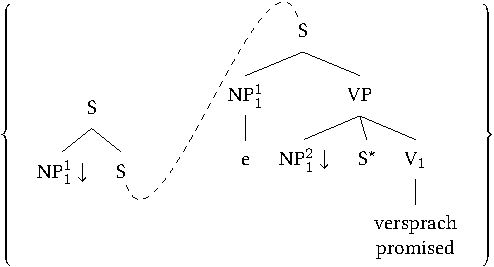
\includegraphics{Figures/tag-versprach-lsp-crop}}

dashed line: The S with the NP$_1^1\downarrow$ sister has to dominate the other S node.

There may be other nodes in between.


}

\frame{


\centerline{%
\scalebox{.75}{
\begin{forest}
tag
[\gruen{S}
	[\gruen{NP$_1^1\downarrow$}]
	[\gruen{S}
		[NP$_2^2\downarrow$]
		[\gruen{S}
			[\gruen{NP$_1^1$}
				[\gruen{e}]]
			[\gruen{VP}
				[\gruen{NP$_1^2\downarrow$}]
				[\gruen{S}
					[NP$_2^1\downarrow$]
					[S
						[NP
							[PRO]]
						[VP
							[NP$_2^1$
								[e]]
							[NP$_2^2$
								[e]]
							[V$_2$
								[zu überführen;to indict]]]]]
				[\gruen{V$_1$}
					[\gruen{versprach};promised]]]]]]
\end{forest}
}}

}

\subsection{Verb position}

\outline{
\begin{itemize}
\item General remarks on the representational format
\item Local reordering (aka scrambling)
\item \alert{Verb position}
\item Passive
\item Long distance dependencies
\item New developments and theoretical variants
\item Summary and classification
\end{itemize}

}

\frame{
\frametitle{Verb position}

\begin{itemize}[<+->]
\item Verb position could be analyzed as in GPSG as linearization variant.
\item Since verb position is relevant for meaning, a lexical rule-based analysis may be more
  appropriate:
\begin{itemize}
\item There are trees for the verb in initial position and in final position.
\item The trees are related by lexical rules.
\item The LRs correspond to transformations in GB:\\
      A verb-final tree is related to a verb-initial tree.
\end{itemize}
\end{itemize}


}



\subsection{Passive}

\outline{
\begin{itemize}
\item General remarks on the representational format
\item Local reordering (aka scrambling)
\item Verb position
\item \alert{Passive}
\item Long distance dependencies
\item New developments and theoretical variants
\item Summary and classification
\end{itemize}

}


\frame{
\frametitle{Passive}


\begin{itemize}[<+->]
\item There is a family of trees for each word.
\item For each active tree there is a passive tree.
\item Trees are related via lexical rules.
\item These lexical rules correspond to transformations of \gb mapping trees onto trees.
\end{itemize}


}

\subsection{Long"=distance dependencies}

\outline{
\begin{itemize}
\item General remarks on the representational format
\item Local reordering (aka scrambling)
\item Verb position
\item Passive
\item \alert{Long distance dependencies}
\item New developments and theoretical variants
\item Summary and classification
\end{itemize}

}


\frame{
\frametitle{Long"=distance dependencies}

\vfill
Trees are inserted into the middle of other trees:
\vfill


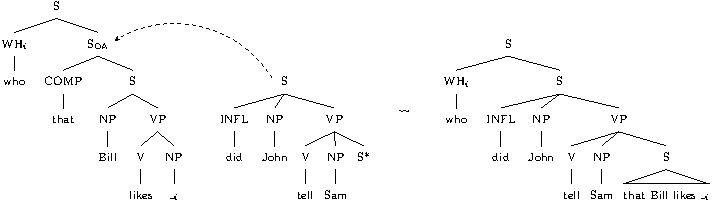
\includegraphics[width=\textwidth]{Figures/tag-long-distance-dependencies-crop}

%% \oneline{%
%% \begin{forest}
%% tag
%% [S
%% 	[WH$_i$
%% 		[who]]
%% 	[%\tikzmark{soa}{S\sub{OA}}
%%          S\sub{OA},name=soa
%% 		[COMP
%% 			[that]]
%% 		[S
%% 			[NP
%% 				[Bill]]
%% 			[VP
%% 				[V
%% 					[likes]]
%% 				[NP
%% 					[\noexpand\_$_i$]]]]]]
%% \end{forest}
%% %}
%% %\hspace{0.5cm}
%% \qquad
%% %\scalebox{.5}{%
%% \begin{forest}
%% tag
%% [S,name=s%\tikzmark{s}{S}
%% 	[INFL
%% 		[did]]
%% 	[NP
%% 		[John]]
%% 	[VP
%% 		[V
%% 			[tell]]
%% 		[NP
%% 			[Sam]]
%% 		[S*]]]
%% \end{forest}
%% %}
%% \qquad \raisebox{2cm}{$\rightsquigarrow$} \qquad
%% %\scalebox{.5}{%
%% \begin{forest}
%% tag
%% [S
%% 	[WH$_i$
%% 		[who]]
%% 	[S
%% 		[INFL
%% 			[did]]
%% 		[NP
%% 			[John]]
%% 		[VP
%% 			[V
%% 				[tell]]
%% 			[NP
%% 				[Sam]]
%% 			[S
%% 				[that Bill likes \noexpand\_$_i$, roof]]]]]
%% \end{forest}
%% \begin{tikzpicture}[overlay,remember picture]
%% \draw[->, dashed, bend angle=45, bend right] ($(pic cs:s)+(-0.25,0.2)$) to($(pic cs:soa)+(0.8,.2)$);
%% \end{tikzpicture}
%% }

\vfill

\eal
\ex \alert{who$_i$} did John tell Sam \alert{that Bill likes \_$_i$}\\
\pause
\ex \alert{who$_i$} did John tell Sam that Mary said \alert{that Bill likes \_$_i$}
\zl

\vfill



}

\frame{
\frametitle{Obligatory adjunction}

\begin{itemize}
\item The tree for \emph{WH COMP NP likes \_$_i$} is a member of the tree family of \emph{likes} and
  hence listed in the lexicon.
\item Although the tree for (\mex{1}) has the category S,\\
      (\mex{1}) is not a well-formed sentence in English.
\ea[*]{
who that Bill likes
}
\z
\pause
Label OA: there has to be an obligatory adjunction at respective nodes.

\end{itemize}


}


\subsection{New developments and theoretical variants}

\outline{
\begin{itemize}
\item General remarks on the representational format
\item Local reordering (aka scrambling)
\item Verb position
\item Passive
\item Long distance dependencies
\item \alert{New developments and theoretical variants}
\item Summary and classification
\end{itemize}

}


\subsubsection{FTAG}

\frame{
\frametitle{Feature-based TAG: FTAG}

\begin{itemize}[<+->]
\item FTAG uses AVMs to describe nodes.
\item Every node consists of two parts, a top one and a bottom one.
\item Exception: substitution nodes. They have just a top structure.
\item The upper structure has to match the node into which it is inserted.
\item For adjunction the upper one has to match the upper node into which it is inserted and the
  lower one the lower node.
\item Pairs are kept till the end of the derivation and then a unification must be possible.
\end{itemize}

}


\frame{
\frametitle{FTAG: Substitution}

\centerline{%
\scalebox{.7}{%
\begin{forest}
tag
[{\ms{
   cat & {\upshape S}\\
 }\\
\ms{
   cat & {\upshape S}
}}
  [\ms{
    cat & {\upshape NP}\\
    agr & \ibox{1}\\
   }
%
   [{[~]\\
    \ms{
       cat & {\upshape NP}\\
       agr & \ms{
              per & 3\\ 
              num & sing\\
             }\\
      }}, substitution,tier=2
      [John, tier=word] ] ]
  [{\ms{
     cat & {\upshape VP}\\
     agr & \ibox{1} \ms{
                    per & 3\\ 
                    num & sing\\
                    }\\
     }\\
     \ms{ 
     cat & {\upshape VP}\\
     }}
     [{\ms{
          cat & {\upshape V}\\
         }\\
       \ms{
          cat & {\upshape V}\\
       }}, tier=2
       [laughs,tier=word]]]
] 
\end{forest}
}\hfill%
\visible<2>{\scalebox{.7}{%
\begin{forest}
tag
[{\ms{
   cat & {\upshape S}\\
 }\\
\ms{
   cat & {\upshape S}
}}
  [{\ms{
    cat & {\upshape NP}\\
    agr & \ibox{1}\\
   }\\
    \ms{
       cat & {\upshape NP}\\
       agr & \ms{
              per & 3\\ 
              num & sing\\
             }\\
      }}
      [John, tier=word] ]
  [{\ms{
     cat & {\upshape VP}\\
     agr & \ibox{1} \ms{
                    per & 3\\ 
                    num & sing\\
                    }\\
     }\\
     \ms{ 
     cat & {\upshape VP}\\
     }}
     [{\ms{
          cat & {\upshape V}\\
         }\\
       \ms{
          cat & {\upshape V}\\
       }}
       [laughs,tier=word]]]
] 
\end{forest}}
}}

\emph{John} is inserted into the substitution node\pause{} and then every top structure has to match every
bottom structure.

}

\frame{
\frametitle{Obligatory adjunction enforced by incompatible features}


\hfill%
%\includegraphics[scale=.6]{Figures/tag-obl-adj-ftag-cropped}
\visible<2->{\scalebox{.6}{%
\begin{forest}
[\rnode{vpone}{\gruen{\ms{
   cat & {\upshape VP}\\
 }}}\vspace{2mm}\\ 
 \ms{
       cat & {\upshape VP}\\
       agr & \ibox{2}\\ 
       mode & ind\\
 }
  [{\ms{
       cat & {\upshape V}\\
      }\vspace{2mm}\\
    \ms{
      cat & {\upshape V}\\
      agr & \ibox{2} \ms{
                      per & 3\\ 
                      num & sing\\
                     }\\
       }} [is]]
  [{\ms{
       cat & {\upshape VP}\\ 
       mode & ger\\
      }\vspace{2mm}\\
    \blau{\ms{
       cat & {\upshape VP}\\
       }$^*$}}]]
\end{forest}}}
%% %%% sings tree:
%% \hspace{-1em}
\hfill
\scalebox{.6}{%
\begin{forest}
for tree={anchor=north} % This used to be in the preamble but was removed there. 09.12.2020 St. Mü.
[{\ms{ 
   cat & {\upshape S}\\
 }\vspace{2mm}\\
 \ms{
  cat & {\upshape S}\\ 
  }}
  [\ms{ cat & {\upshape NP}\\
        agr & \ibox{1}\\
      }]
  [\rnode{vptwo}{\gruen{\ms{
      cat  & {\upshape VP}\\
      agr  & \ibox{1}\\
      mode & ind\\
      }}}\vspace{2mm}\\
     \blau{\ms{
     cat & {\upshape VP}\\ 
     mode & ger\\
     }}
     [{\ms{ cat & {\upshape V}\\
          }\vspace{2mm}\\
       \ms{
            cat & {\upshape V}\\
        }}
       [laughing]]]]
\end{forest}
%\begin{tikzpicture}[overlay,remember picture,out=0,in=220]
%\draw[->, dashed] (vpone) to (vptwo);
%\end{tikzpicture}
}
\visible<2->{\nccurve[angleA=-15,angleB=-140,linestyle=dashed]{->}{vpone}{vptwo}}
\hfill\hfill
\visible<3>{\scalebox{.6}{%
\begin{forest}
for tree={anchor=north}
[{\ms{ 
   cat & {\upshape S}\\
 }\vspace{1mm}\\
  \ms{
   cat & {\upshape S}\\
  }}
  [{\ms{ cat & {\upshape NP}\\
         agr & \ibox{1}\\
   }}]
  [\gruen{\ms{
     cat  & {\upshape VP}\\
     agr  & \ibox{1}\\
     mode & ind\\
    }}\vspace{1mm}\\
    \gruen{\ms{
       cat & {\upshape VP}\\
       agr & \ibox{2}\\ 
       mode & ind\\
    }}
    [{\ms{
       cat & {\upshape V}\\
      }\vspace{1mm}\\
      \ms{
        cat & {\upshape V}\\
        agr & \ibox{2} \ms{
                per & 3\\ 
                num & sing\\
               }\\
         }} [is]]
     [\blau{\ms{
        cat & {\upshape VP}\\ 
        mode & ger\\
      }}\vspace{1mm}\\
      \blau{\ms{
       cat & {\upshape VP}\\ 
       mode & ger\\
      }}
      [{\ms{ cat & {\upshape V}\\
           }\vspace{1mm}\\
        \ms{
             cat & {\upshape V}\\
        }} [laughing]]]]]
\end{forest}
}}\hfill\hfill\mbox{}
}



\subsection{Summary and classification}

\outline{
\begin{itemize}
\item General remarks on the representational format
\item Local reordering (aka scrambling)
\item Verb position
\item Passive
\item Long distance dependencies
\item New developments and theoretical variants
\item \alert{Summary and classification}
\end{itemize}

}


\frame{
\frametitle{Idioms in TAG}

Idioms are really simple \citep{AS89a}:

\centerline{
\scalebox{.9}{%
\begin{forest}
tag
[S
	[NP$\downarrow$]
	[VP
		[V
			[takes]]
		[NP$\downarrow$]
		[PP$_{{\mathrm{NA}}}$
			[P
				[into]]
			[NP$_{\mathrm{NA}}$
				[N$_{\mathrm{NA}}$
					[account]]]]]]
\end{forest}
}}

\pause
This is the perfect Construction Grammar (and it is lexicalized!)!


}

\frame{
\frametitle{Summary}

\begin{itemize}
\item L-TAG is really simple:
\begin{itemize}
\item lexically anchored trees
\item two combination operations
\end{itemize}
\pause
\item recursion is filtered out of trees
\pause
\item no empty elements in the lexicon but in the trees
\pause
\item various extensions of the core formalism (multi-component, feature-based)
\end{itemize}


}



%      <!-- Local IspellDict: en_US-w_accents -->
